% Created 2021-02-06 Sat 17:14
% Intended LaTeX compiler: pdflatex
\documentclass[11pt]{article}
\usepackage[utf8]{inputenc}
\usepackage[T1]{fontenc}
\usepackage{graphicx}
\usepackage{grffile}
\usepackage{longtable}
\usepackage{wrapfig}
\usepackage{rotating}
\usepackage[normalem]{ulem}
\usepackage{amsmath}
\usepackage{textcomp}
\usepackage{amssymb}
\usepackage{capt-of}
\usepackage{hyperref}
\author{Tigany Zarrouk\thanks{tigany.zarrouk@kcl.ac.uk}}
\date{23.02.2021}
\title{Multi-scale investigation of dislocation assisted carbon migration in ferrite}
\hypersetup{
 pdfauthor={Tigany Zarrouk},
 pdftitle={Multi-scale investigation of dislocation assisted carbon migration in ferrite},
 pdfkeywords={},
 pdfsubject={},
 pdfcreator={Emacs 27.1 (Org mode 9.4.4)}, 
 pdflang={English}}
\begin{document}

\maketitle

\section*{Introduction}
\label{sec:orgcb97641}
\begin{itemize}
\item Rolling contact on bearing raceways generate maximal shear
stresses in subsurface.
\item Degradation of subsurface microstructure observed.
\item This can lead to failure by Rolling Contact Fatigue (RCF).
\item Subsurface degradation arises in form of Dark
Etching Regions (DERs).
\item DERs characterised by development of ferrite and carbide features with
patches of unaltered martensitic matrix.
\end{itemize}
\begin{figure}[htbp]
\centering
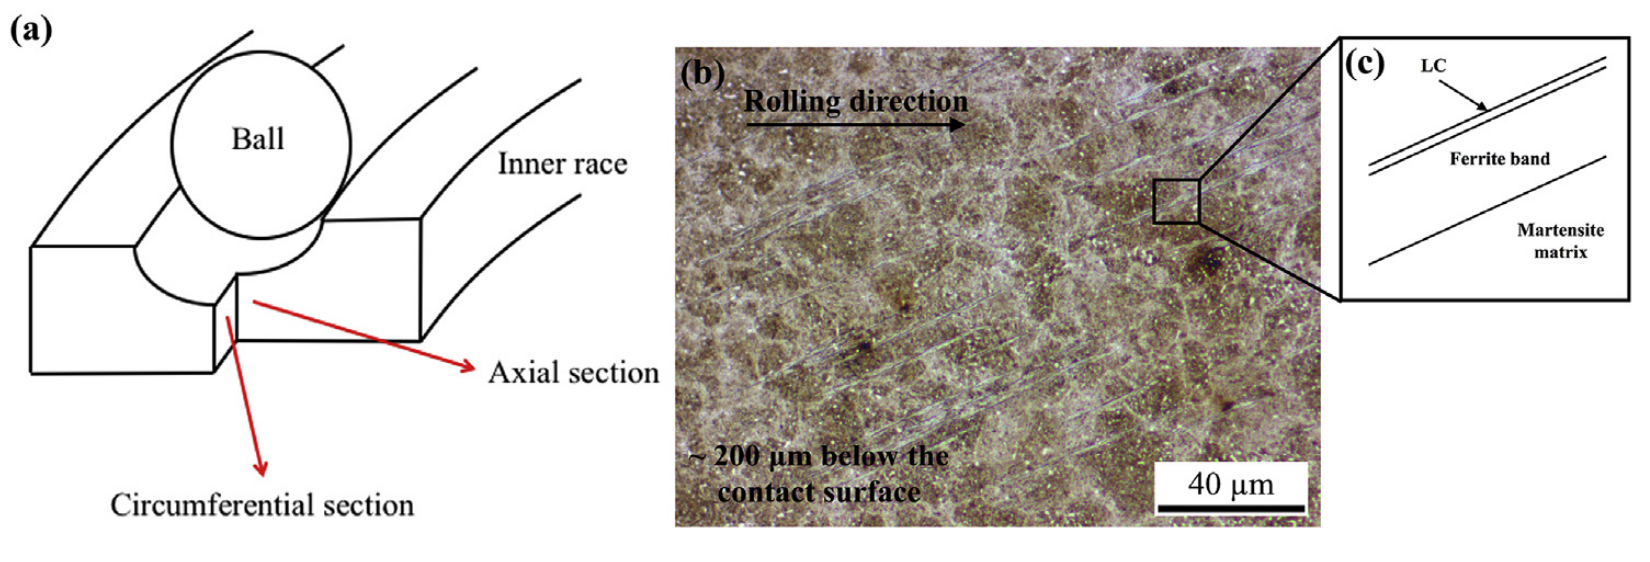
\includegraphics[width=.9\linewidth]{/home/tigany/Documents/docs/Management/fe_skf_paper/sebastian/Images/der_picture_fu.png}
\caption{\label{fig:org2f48977}Diagram of DER location within a bearing and its characteristics, \cite{Fu2017} \label{fuderpicture}}
\end{figure}


\section*{Motivation}
\label{sec:orgb94488b}
\begin{itemize}
\item Carbon redistribution and plastic deformation are thought to be
fundamental mechanisms behind DER formation.
\item Differing mechanisms of dislocation-driven carbon migration have
been suggested, but no consensus.
\item Atomistic modelling necessary to elucidate how dislocations could
move carbon; thus clarifying potential mechanisms of DER formation.
\end{itemize}

\section*{Aims}
\label{sec:orgfb3a83d}
To answer the questions:
\begin{itemize}
\item How can dislocations assist in carbon migration?
\item How are dislocations influenced by carbon on atomistic scale?
\begin{itemize}
\item Is dislocation core structure affected?
\item How does carbon affect kink-pair nucleation/migration?
\end{itemize}
\end{itemize}

\section*{Methods}
\label{sec:org29ec1b3}
\begin{itemize}
\item Quantum-mechanical tight-binding simulations used to determine
influence of atomistic carbon on dislocations (more accurate than
empirical potentials, better scaling than DFT).
\item Line tension model of dislocation to acquire stress-dependent
kink-pair formation energies.
\item Future work is to use kMC model to see what happens at even larger
scale of large-scale dislocation movement.
\end{itemize}
\begin{center}
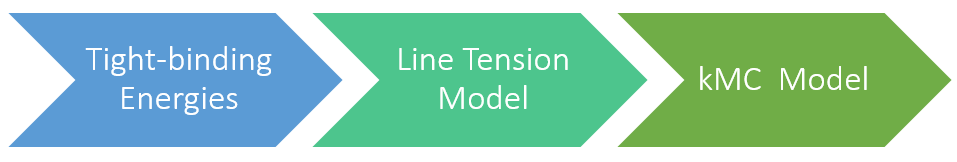
\includegraphics[width=.9\linewidth]{/home/tigany/Documents/docs/Management/Images/skf_process_tb_lt_kmc.PNG}
\label{org61f731b}
\end{center}


\section*{Tight-binding}
\label{sec:org9b29a0b}
Cell dislocaton arrangement used to find Peierls potential.
Simulation cell used to find binding energies of carbon to screw dislocations.




\subsection*{Peierls Potential}
\label{sec:org8b7656c}
DFT Peierls potential of screw dislocation.
Tight-binding Peierls potential of screw dislocation.



\subsection*{Binding of C to screw core}
\label{sec:orgeef6e51}

\begin{itemize}
\item Distribution of carbon around the easy core dislocation.
\end{itemize}
\begin{itemize}
\item Distribution of carbon around the hard core dislocation.
\item The first and second closest octahedral sites to the hard core decay to a prismatic position inside the hard core.
\end{itemize}


\section*{Carbon concentration on dislocation line}
\label{sec:org3cc3c3f}
\begin{itemize}
\item Can solve for the equilibrium carbon concentration on the
dislocation line from the Fe-C binding energies around the
dislocation core.
\item Can include the effect of the C-C first-neighbour repulsive
energy, which reduces the overestimation from using the bare
McClean Isotherm for the equlilbrium concentration.

\begin{equation}
\end{itemize}
\frac\{ c\textsubscript{d}\textsuperscript{i} \}\{1 -  c\textsubscript{d}\textsuperscript{i} \} = \frac\{ c\textsubscript{\text{bulk}} \}\{1 - c\textsubscript{\text{bulk}} \} \text{exp} \Big(
  \frac\{E\textsubscript{\text{b}}\textsuperscript{i}\}\{k\textsubscript{\text{B}}T\}  \Big)
  \end{equation}

\begin{equation}
N_{\text{oct}}    c_{\text{bulk}} + N_d c_d = N_{\text{oct}} c_{\text{nom}}/3
\end{equation}




\section*{Line tension}
\label{sec:orgf7c8b9f}

\[ E_{\text{LT}} = \frac{K}{2} \sum_j (\vec{P}_j - \vec{P}_{j+1} )^2  + \sum_j \Delta E_{\text{P}}  (\vec{P}_j) +
   (\sigma \cdot \vec{b}) \times \vec{l} \cdot \vec{P}_j  - \sum_{j,k} E_{\text{C}} (|\vec{P}_j-\vec{P}_k^{\text{C}}|), \]

\begin{itemize}
\item Equation used for the line tension model.
\item The interaction between solutes is parameterised with a
lorentzian.
\end{itemize}


\subsection*{Kink-pair formation enthalpies}
\label{sec:org5931b9d}

\begin{center}
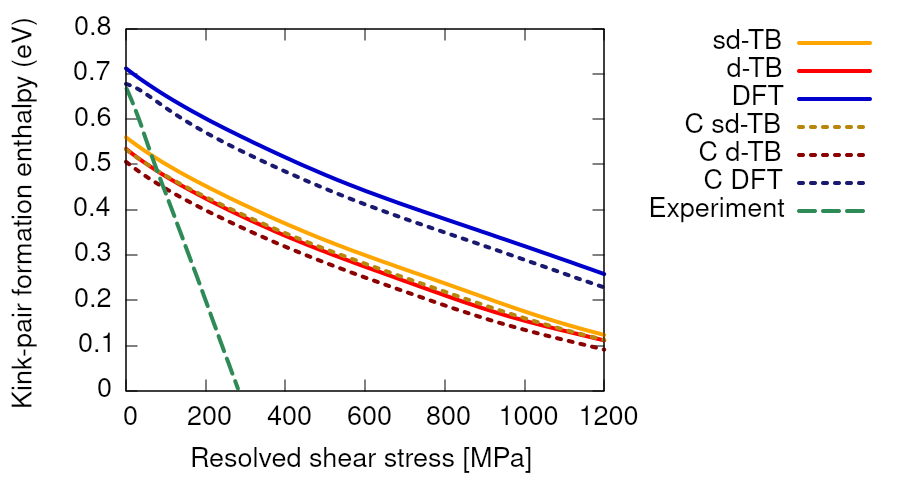
\includegraphics[width=.9\linewidth]{/home/tigany/Documents/docs/Management/fe_skf_paper/sebastian/Images/kink-pair_formation_enthalpies_just_results.png}
\end{center}

\begin{itemize}
\item The addition of carbon reduces the kink-pair formation enthalpy.
\item The reduction is less than one would expect from hydrodgen as the
interaction with carbon is longer ranged due to the large
tetragonal distortion and binding energies.
\end{itemize}

\section*{Summary}
\label{sec:orgdca35e9}
\begin{itemize}
\item Obtained Peierls potential and binding energies of carbon distributed around hard and easy screw
dislocation cores from quantum-mechanical atomistic simulations.
\item Calculated the equilibrium concentration of carbon on the
dislocation line by calculation of C-C repulsive energies.
\item Find that \textbf{all} dislocations are hard core, at typical dislocation densities,
nominal carbon concentrations and temperatures, due to the
reconstruction of easy core due to carbon-dislocation interaction
and operating temperatures.
\item Carbon decreases the stress necessary to move the screw
dislocations at all temperatures.
\end{itemize}
\end{document}
